% 2013 全国卷Ⅱ文科第 22 题：外接圆、切线及过 B,E,F,C 的圆。
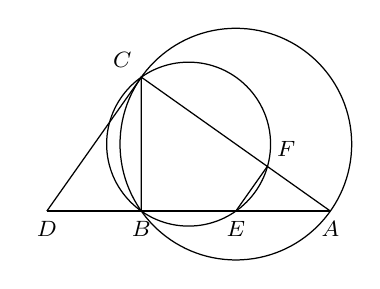
\begin{tikzpicture}[font=\footnotesize, line width=0.45pt]
  \coordinate (B) at (0,0);
  \coordinate (E) at (1.20,0);
  \coordinate (A) at (2.40,0);
  \coordinate (D) at (-1.20,0);
  \coordinate (C) at (0,1.70);
  \coordinate (F) at (1.60,0.567);
  \coordinate (O) at (1.20,0.85);
  \coordinate (o) at (0.60,0.85);
  \draw (O) circle[radius=1.471];
  \draw (o) circle[radius=1.041];
  \draw (D)--(A);
  \draw (D)--(C);
  \draw (B)--(C)--(A);
  \draw (E)--(F);
  \node[below] at (D) {$D$};
  \node[below] at (B) {$B$};
  \node[below] at (E) {$E$};
  \node[below] at (A) {$A$};
  \node[above left] at (C) {$C$};
  \node[above right] at (F) {$F$};
\end{tikzpicture}
